
%(BEGIN_QUESTION)
% Copyright 2010, Tony R. Kuphaldt, released under the Creative Commons Attribution License (v 1.0)
% This means you may do almost anything with this work of mine, so long as you give me proper credit

Suppose we have an Allen-Bradley SLC 500 controller connected to a pair of momentary-contact pushbutton switches and contactor controlling power to an electric motor as shown in this illustration:

$$\includegraphics[width=15.5cm]{i04069x01.eps}$$

This motor control system has a problem, though: the motor refuses to start when the ``Start'' pushbutton is pressed.  Closely examine the pictorial diagram (including the status LEDs on the PLC's I/O cards), then identify at least two faults that could account for the motor's refusal to start.

\vskip 20pt \vbox{\hrule \hbox{\strut \vrule{} {\bf Suggestions for Socratic discussion} \vrule} \hrule}

\begin{itemize}
\item{} A helpful problem-solving tip is to note the PLC's I/O states by examining the LED indicators on each input and output card on the PLC rack.  What do the LED states tell you in this particular example?
\end{itemize}

\underbar{file i04069}
%(END_QUESTION)





%(BEGIN_ANSWER)


%(END_ANSWER)





%(BEGIN_NOTES)

Looking at the input card's LED indicators, we see input 4 (the OL contact) is energized as it should be, but the ``Stop'' pushbutton's input IN2 is not energized as it should be (since the real-world pushbutton is NC and no one is pressing the button).

\vskip 10pt

Some possible faults:

\begin{itemize}
\item{} Stop pushbutton switch failed open
\item{} Wire between terminal 8 and pushbutton switches failed open
\item{} Wire between stop pushbutton and terminal IN2 failed open
\item{} Input channel IN2 failed open
\end{itemize}




\vskip 20pt \vbox{\hrule \hbox{\strut \vrule{} {\bf Virtual Troubleshooting} \vrule} \hrule}

This question is a good candidate for a ``Virtual Troubleshooting'' exercise.  Presenting the diagram to students, you first imagine in your own mind a particular fault in the system.  Then, you present one or more symptoms of that fault (something noticeable by an operator or other user of the system).  Students then propose various diagnostic tests to perform on this system to identify the nature and location of the fault, as though they were technicians trying to troubleshoot the problem.  Your job is to tell them what the result(s) would be for each of the proposed diagnostic tests, documenting those results where all the students can see.

During and after the exercise, it is good to ask students follow-up questions such as:

\begin{itemize}
\item{} What does the result of the last diagnostic test tell you about the fault?
\item{} Suppose the results of the last diagnostic test were different.  What then would that result tell you about the fault?
\item{} Is the last diagnostic test the best one we could do?
\item{} What would be the ideal order of tests, to diagnose the problem in as few steps as possible?
\end{itemize}

%INDEX% PLC, troubleshooting: motor start/stop control circuit

%(END_NOTES)


